\documentclass{VUMIFInfBakalaurinis}
\usepackage{algorithmicx}
\usepackage{algorithm}
\usepackage{algpseudocode}
\usepackage{amsfonts}
\usepackage{amsmath}
\usepackage{bm}
\usepackage{caption}
\usepackage{color}
\usepackage{float}
\usepackage{graphicx}
% \usepackage{hyperref}  % Nuorodų aktyvavimas
\usepackage{listings}
\usepackage{subfig}
\usepackage{url}
\usepackage{wrapfig}

% Titulinio aprašas
\university{Vilniaus universitetas}
\faculty{Matematikos ir informatikos fakultetas}
\department{Programų sistemų katedra}
\papertype{Baigiamasis bakalauro darbas}
\title{Privačios informacijos išsaugojimas taikant dirbtinio intelekto technologijas}
\titleineng{Privacy-preserving AI}
\status{4 kurso 3 grupės studentas}
\author{Paulius Milmantas}
\supervisor{dr. Linas Petkevičius}
\date{Vilnius \\ \the\year}

% Nustatymai
% \setmainfont{Palemonas}   % Pakeisti teksto šriftą į Palemonas (turi būti įdiegtas sistemoje)
 \bibliography{bibliografija}

\begin{document}
\maketitle

\tableofcontents

\sectionnonum{Įvadas}
	%(https://eur-lex.europa.eu/legal-content/LT/TXT/?uri=celex%3A32016R0679)	
	\par Mašininis mokymas yra dirbtinio intelekto sritis, kuri pasitelkia statistinius algoritmus, kad apibrėžtų duomenų atpažinimo modelį. Modelio apmokymui dažniausiai reikia turėti daug duomenų. Kai kurie uždaviniai reikalauja duomenų, kurie nėra laisvai prieinami ir yra privatūs. Mašininio mokymo tyrimų srityje yra kilusi problema dėl jų saugojimo. Vienas iš faktorių, kuris lėmė šį susidomėjimą yra 2016 metais Europoje priimtas duomenų apsaugos reglamentas (GDPR). Pagal jį, fizinių asmenų duomenys turi būti saugomi naudojantis tam tikromis taisyklėmis ir negali būti atskleisti trečiosioms šalims, be asmens sutikimo \cite{1}.
	% https://towardsdatascience.com/perfectly-privacy-preserving-ai-c14698f322f5
	\par Šią problemą išspręsti siekia įvairūs tyrimai ir naujai atrasti metodai privatumą saugančio dirbtinio intelekto srityje. Šią problemą galima išskaidyti į kelias atskiras sritis:
\begin{itemize}
    \item Analizuojamų duomenų privatumas \cite{2}. Algoritmas apmoko modelį atpažinti duomenis. Turint sukurtą modelį, neturi būti galima atgaminti duomenų, pagal kuriuos jis buvo mokomas, bei negali būti identifikuoti asmenys. Taip nukentėtų žmonių privatumas ir būtų pažeistas Europos duomenų apsaugos reglamentas. Šio pažeidimo pavyzdys gali būti ir paprastas teksto atkūrimo modelis. Duodama sakinio pradžia, modelis nuspėja jo pabaigą. Jeigu suvedus tam tikras detales modelis užbaigia sakinį naudodamas asmeninius duomenis, kurie atskleidžia žmonių tapatybę, šis modelis nėra saugus.
    \item Duomenų įvesties privatumas \cite{2}. Trečios šalys neturi matyti įvedamų duomenų. Tai gali būti tinklo saugumo spragos, duomenų surinkimo aplikacijų spragos ir t.t…
    \item Modelio išvesties privatumas \cite{2}. Modelio išvesties neturi matyti asmenys, kuriems šie duomenys nepriklauso. Šis punktas yra sąlyginis, priklauso nuo modelio svarbos. Jeigu tai yra svarbūs asmeniniai duomenys, negalima rizikuoti. Tačiau jeigu tai yra viešai prieinami duomenys, šis punktas negalioja.
    \item Modelio apsauga \cite{2}. Sukurtas modelis negali būti niekieno pasisavintas. Šis punktas yra skirtas apsaugoti programos kūrėją.
\end{itemize}
	% https://www.nature.com/articles/s42256-020-0186-1
	% https://towardsdatascience.com/the-new-dawn-of-ai-federated-learning-8ccd9ed7fc3a
	\par Darbo tikslas - ištirti ir palyginti privatumą saugančius dirbtinio intelekto algoritmus pagal jų saugumą, našumą ir panaudojamumą.
	\par Darbo uždaviniai:
	\begin{itemize}
		\item Išanalizuoti esamus algoritmus pagal jų saugumą ir panaudojamumą.
		\item Ištirti kurie algoritmai yra realizuoti ir dalį nerealizuotų, realizuoti.
		\item Palyginti algoritmus pagal našumą. 
	\end{itemize}
\section{Asmens duomenų privatumas mašininio mokymo kontekste}
	\par Vienas iš būdų apsaugoti duomenis yra decentralizuoti modelį ir naudoti paskirstyto mokymo algoritmus. Paprastai mašininiam mokymui yra naudojamas centralizuotas serveris. Yra surenkami duomenys į vieną vietą ir modelį moko vienas kompiuteris. Jeigu norima pridėti daugiau duomenų arba papildomą klasifikatorių, modelį reikia apmokyti iš naujo. Taip pat, kas kuria šį modelį, turi visą prieigą prie duomenų, šie modeliai nėra saugūs. 
	\par Šiai bėdai išspręsti, vienas iš metodų yra federuotas mašininis mokymas (\enquote{Federated machine learning}). Šis metodas padeda išspręsti kaikurias bėdas, vykdant modelio mokymą decentralizuotai \cite{3}. Prie bendro tinklo gali prisijungti daug įrenginių. Visi jie turi savo unikalų duomenų rinkinį. Kiekvienas įrenginys pasirenka geriausią statistinį metodą modelio mokymui ir jį sukurią. Taip yra sukuriama daug skirtingų modelių su skirtingais duomenų rinkiniais. Visi šie rinkiniai vėliau yra surenkami į vieną vietą ir toliau naudojami duomenų analizei. Taip surinkus atskirų įrenginių sukurtus modelius, neturime prieigos prie duomenų ir daugiau žmonių gali prisidėti prie modelio kūrimo, nematant pilno duomenų rinkinio. Tačiau naudojant šį metodą ne visos problemos yra išsprendžiamos. Duomenų saugumas nėra garantuojamas \cite{3}. Jeigu duomenys nėra užšifruojami, jie gali būti pavogti. Tai gali būti padaryta, jeigu yra naudojamas nesaugus interneto ryšys, arba jeigu yra bandoma analizuoti atskirų įrenginių atsiųstus modelius. Šis metodas išsprendžia tik kelias problemas. Likusios yra: komunikavimo kaštai, įrenginių heterogeniškumas, statistinis heterogeniškumas ir saugumo problemos \cite{4}.
%https://www.researchgate.net/publication/335319008_Federated_Learning_Challenges_Methods_and_Future_Directions
	\par Visos šios problemos yra nagrinėjamos ir joms spręsti kuriami nauji metodai. Komunikacijos kaštams mažinti, yra kuriami algoritmai, kaip turi būti perduodamas modelis tinkle, kad būtų maža tinklo apkrova. Įrenginių heterogeniškumui spręsti, yra parenkami tam tikri įrenginių rodikliai ir pagal tai nustatoma, kokia bus įrenginio komunikacija: ar jis naudos asinchroninį komunikavimą, kaip dažnai tai vyks ir kokia yra įrenginio klaidos tikimybė \cite{4}. Statistikos heterogeniškumui pataisyti kuriami yra metodai, kaip meta duomenų-mokymas ir keletos užduočių mokymas (\enquote{Multi-task learning}) \cite{4}. 
	% https://arxiv.org/pdf/1906.10893.pdfmif
	\par Straipsnyje apie privatumą išsaugančius blokų-grandinių tinklus (\enquote{Privacy-Preserving Blockchain-Based Federated Learning for IoT Devices}) yra pateikiamas naujas paskirstyto mokymosi algoritmas, kuris yra paremtas
blokų grandinių technologijomis \cite{5}. Šis modelis yra grafiškai pateiktas pav.1. Šią architektūrą pavyzdyje sudaro 3 komponentai: gamintojai, klientai ir "block chain" tinklas. Šiame pavyzdyje gamintojas pareiškia užklausą, kad reikia atlikti apklausą. Klientai, kurie sutinka su užklausa, išsiunčia savo sukurtą modelį. "Block chain" tinklas elgiasi kaip centralizuotas serveris ir surenka visus klientų modelius. Tuomet, pasirinktas kompiuteris, kuris atlieka visą darbą (\enquote{miner}) atlieka galutinį modelių sujungimą.


\begin{figure}[ht]
  \centering
  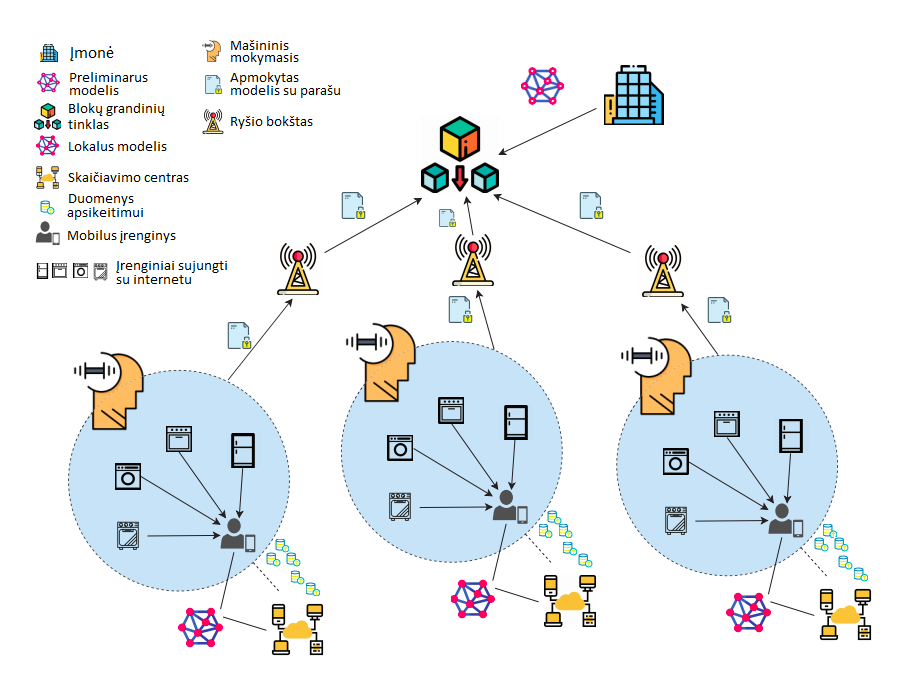
\includegraphics[width=13cm,height=11cm,keepaspectratio]{img/paskirstytasMokymasis.png}
  \caption{Paskirstytas mokymas \cite{5}}
  \label{fig:overflowProblem}
\end{figure}

% https://www.inpher.io/technology/what-is-secure-multiparty-computation
\par Minėti decentralizuoti būdai apjungia skirtingus sukurtus modelius į vieną ir visi įrenginiai kurie kuria modelius, naudoja savo unikalius duomenis. Saugus skirtingų pusių skaičiavimo metodas (\enquote{Secure multiparty computation}) yra kriptografinis protokolas, kuris leidžia įrenginiams, su unikaliais duomenimis, skaičiuoti funkcijos reikšmę, nematant kitų įrenginių reikšmių \cite{6}. Su šiuo metodu, yra sukuriamas vienas modelis tarp įvairių įrenginių. Pagrindinis įrenginys, kuris ruošia skaičiavimo užklausą, gali suskaidyti pradinius duomenis, užšifruoti juos ir taip paskirstyti tarp kitų įrenginių. Taip sukurti įrenginio rezultatai negali būti atšifruoti ir pasisavinti, o minėto federuoto mokymo metodo sukurti rezultatai, jeigu nėra gerai apsaugoti, gali būti pasisavinti ir atgauti pradiniai duomenys su kuriais modelis buvo sukurtas.
% https://www.researchgate.net/publication/236935821_Homomorphic_Encryption_Theory_Applications
\par  Kitas būdas apsaugoti modelį yra naudoti homomorfinį šifravimą. Pagal šį metodas, modelis yra mokomas naudojant užšifruotais duomenimis. Jie mokymo metu, nėra atšifruojami. Šis metodas leidžia keliems įrenginiams vienu metu atlikti skaičiavimus su duomenimis, kurių jie nemato. Yra daug metodo varijacijų. Kaikurios yra pažeidžiamos ir gali atskleisti visos infrastruktūros duomenis \cite{7}. Dažniausiai homomorfinės sistemos yra labiau pažeidžiamos nei nehomomorfinės \cite{7}.
% https://eprint.iacr.org/2016/421.pdf
\par 2016 metais buvo pasiūlytas naujas metodas paspartinti pilnai homomorfines šifravimo sistemas \cite{8}. Homomorfinės sistemos, kurios naudoja šį metodą yra laikomos ketvirtos kartos. Šis metodas leidžia aproksimuoti užšifruoto teksto sudėtį, daugybą ir pakeisti atšifruoto teksto proporcijas \cite{8}. 
Proporcijų pakeitimo procedūra suskaido užšifruotą tekstą į dalis, to pasekoje yra apvalinamas neužšifruotas teksas. Šio metodo pagrindinė idėja yra pridėti triukšmo prie pagrindinės žinutės. Šis triukšmas yra pridedamas prie neužšifruoto teksto dėl saugumo priežasčių ir jis yra laikomas kaip aproksimavimo paklaida. Tuo pasekoje, metodas veikia su tam tikra paklaida
% https://www.inpher.io/technology/what-is-secure-multiparty-computation
\par Bendro įspūdžio agregavimo metodas yra naujausias iš visų minėtų. Jis leidžia įrenginiui su savo duomenimis sukurti modelį naudojant betkokius metodus ir taip prisidėti prie bendro progreso \cite{6}. Visi modeliai yra surenkami ir leidžiami duomenys per šiuos modelius. Kiekvienas modelis skiria savo balsą, jie surenkami ir padaromas bendras sprendimas. Šis metodas leidžia lengvai plėsti modelį. Taip pat yra saugomas ir duomenų privatumas. Jeigu keli modeliai, kurie nesidalina duomenimis, teigia vienodai, tai reiškia, kad negalima atkurti duomenų ir jie yra saugūs \cite{6}. Skaičiavimas vykdomas pasirenkant optimalią strategiją ir imant mažiausią galimą žingsnių skaičių.












%https://www.researchgate.net/publication/335319008_Federated_Learning_Challenges_Methods_and_Future_Directions – kylančios problemos




	%https://www.researchgate.net/publication/236935821_Homomorphic_Encryption_Theory_Applications
	












%Idomus straipsnis apie block chain technologijas
%https://arxiv.org/pdf/1906.10893.pdf

%Apie galimybe nulauzti modeli
%https://arxiv.org/abs/1911.07135







\section{Pažeidžiamumo metrikos}

\par Norint apsaugoti duomenis, sukurtam duomenų aptikimo modeliui reikia atlikti analizę, kaip tikėtina, kad modelio pradiniai duomenys bus atkurti. Tai išanalizuoti yra daug būdų, vienas iš jų yra pateiktas straipsnyje \cite{9}.
 Šis straipsnis ieško metrikos reikšmės, kuri parodo, kaip pradinius duomenis atsimena modelis.
\par Tarkime turime duomenų rinkinį s[r]. Šiam rinkiniui pirma reikia apskaičiuoti rangą \cite{8}.

\begin{equation}
rangas(s[r]) = | {r` \in R : Px(s[r`]) \leq Px(s[r])} |
\label{eq:Lygtis 1.}
\end{equation}

\par Šis rangas nurodo, kurioje vietoje yra šis inicijuotas duomenų rinkinys sąraše, tarp visų galimų testinių rinkinių kombinacijų. \textbf{[TODO: Įterpti pavyzdį]}
\par Rangas tiesiogiai nepasako kokia yra tikimybė, kad bus sugeneruotas toks testavimo rinkinys. Jo skaičiavimas paima daug resursų, nes reikia sugeneruoti visas galimas kombinacijas \cite{8}.
\par Kitas nagrinėjamas kintamasis yra \enquote{atvirumo} metrika. Tai aproksimuotas skaičius, kuris nusako, kaip tikėtina, jog testavimo duomenys bus atgaminti iš modelio. Ši metrija pasako ką naujo sužinome apie pradinius duomenis, kai per modelį paleidžiame atsitiktinai sugeneruotus duomenis. Todėl, reikia skaičiuoti spėjimo entropijos redukcijos lygtį. Spėjimo entropija, tai spėjimų skaičius E(X), kuris reikalingas atspėti diskretų, atsitiktinai sugalvotą parametrą X \cite{8}. 
\par Jeigu kintamasis r yra pasirenkamas atsitiktinai r \in R, tai reiškia, kad reikia generuoti atsitiktinius skaičius tol, kol bus gauta r reikšmė. Iš to seka, kad spėjimų turėtų būti lygus 2 lygčiai.

\begin{equation}
E(s[r])_{\thera} = \frac{1}{2}| R |
\label{eq:lygtis2}
\end{equation}

\textbf{[TODO: Pridėti lygties išvedimą]}

\begin{equation}
atvirumas(s[r])_{\theta} = \log_2 | R | - \log_2 rangas_{\theta}(s[r])

\end{equation}




\section{Modelio duomenų atgavimo metodai}

\section{Homomorfinis šifravimas}

\section{Federuotas mašininis mokymas}
\subsection{Metodas}
\subsection{Komunikacijos kaštų mažinimas}
\subsection{Įrenginių heterogeniškumas}
\subsection{Analizės heterogeniškumas}
\subsection{Saugos problemos}

\section{Blokų-grandinių technologija}

\section{Saugus skirtingų pusių skaičiavimas}

\section{Bendro įspūdžio privatus agregavimas}




\printbibliography[heading=bibintoc]


\end{document}
